\chapter{Zero-Knowledge Linear Code}

In this chapter, we use the construction presented in paper \cite{10.1145/2554797.2554815} to add a zero-knowledge property to a normal linear code through code transformation. 

% http://www.cs.cmu.edu/~odonnell/toolkit13/lecture12.pdf
\section{Random d-regular Bipartite Graph}
\label{sec:randomgraph}
First, we present an algorithm to generate a random d-regular bipartite graph. To make sure each vertex has degree $d$, we can first sample $d$ random perfect matching for 2 sets of $n$ vertices. Then take the union of them. Note that it is possible to generate parallel edges. But this should not be a concern for our purpose here. And it can be shown that this happens with low probability.

\RestyleAlgo{ruled}
%% This is needed if you want to add comments in
%% your algorithm with \Comment
\SetKwComment{Comment}{/* }{ */}
\begin{algorithm}[hbt!]
\caption{Random d-regular Bipartite Graph Generation}
\label{alg:randomgarph}
\KwData{$n \geq 0$, $d <= n$}
\KwResult{A random $d$-regular bipartite graph $G=(L, R, E)$ with $|L| = |R| = n$}

$L \gets \text{a set of } n \text{ nodes}$\;
$R \gets \text{a set of } n \text{ nodes}$\;
$E \gets \emptyset$\;
$P \gets [1, 2, \cdots , n]$\;
\For{$i$ in $1, 2, \cdots , d$}{
    Permute $P$ randomly \Comment*[r]{sample a perfect matching}
    \For{$j$ in $1, 2, \cdots , n$}{
        $E \gets E \cup (L_j, R_{P_j})$ \;
    }
}
\Return{(L, R, E)}
\end{algorithm}


\section{Expander Graph}

\begin{lemma}
\label{lemma:randomgraph}

For any $0 < \epsilon < 1$, there exist a degree $d$ such that a random $d$-regular bipartite graph $G=(L, R, E)$ with $|L| = |R| = n$ generated according to algorithm \ref{alg:randomgarph} satisfy the following property with high probability.

    \begin{itemize}
        \item Expansion: For every set $X \subset L$ with $|X| \ge \epsilon n$, if $Y$ is the set of neighbors of $X$ in $G$, then $|Y| \ge (1 - \epsilon)  n$.
    \end{itemize}

\end{lemma}

\begin{proof}

Negating the statement, we can say that the randomly generated graph $G$ does not satisfy the expansion property if and only if $\exists S \subseteq L$, $|S| \ge \epsilon n$, $\exists M \subseteq R$, $|M| \ge  \epsilon n$ such that there is no edge connecting between set $S$ and set $M$. We bound the probability that this negating statement is true as follows:

For every vertex $a \in L$ and every vertex $b \in R$, the probability that $a$ and $b$ are not connected in the random graph $G$ is:

$$P_1 = (\frac{n-1}{n})^{d}$$

For a set of vertices, $S \subset L$ with $|S| = s \ge \epsilon n$, the probability that non of the vertices in $S$ is connected to $b$ is:

$$P_2 = (P_1)^s = (\frac{n-1}{n})^{d s}$$

The probability that there exists at least $\epsilon n$ vertices in $R$ that are not connected to any vertex in $S$ is:

$$P_3 = \binom{n}{\epsilon n} (P_2)^{\epsilon n} = \binom{n}{\epsilon n} (\frac{n-1}{n})^{d s \epsilon n}$$

For $0 \le x \le 1$, we denote the binary entropy function to be:

$$H(x) = -x\log_2 x - (1-x)\log_x (1-x)$$ 
where we adopt the convention that $0 \log_2 0 = 0$.

Then, we take a union bound over all possible sets $S$, 

\begin{align}
% bound 5
P_4 &= \sum_{s=\epsilon n}^{n} \binom{n}{s} P_3 \nonumber \\
    &= \sum_{s=\epsilon n}^{n} \binom{n}{s} \binom{n}{\epsilon n} (\frac{n-1}{n})^{d s \epsilon n} \nonumber \\
    &\le \sum_{s=\epsilon n}^{n} \binom{n}{s} \binom{n}{\epsilon n} (\frac{n-1}{n})^{d \epsilon^2 n^2} 
    && \text{since } s \ge \epsilon n \text{ and } \frac{n-1}{n} < 1 \nonumber \\
    &\le \sum_{s=\epsilon n}^{n} \binom{n}{s} 2^{n H(\frac{\epsilon n}{n})} (\frac{n-1}{n})^{d \epsilon^2 n^2} 
    && \binom{n}{k} \le 2^{n H(\frac{k}{n})} \nonumber \\
    &= \sum_{s=\epsilon n}^{n} \binom{n}{s} 2^{n H(\epsilon)} ((1 - \frac{1}{n})^{n})^{d \epsilon^2 n} \nonumber \\
    &\le \sum_{s=\epsilon n}^{n} \binom{n}{s} 2^{n H(\epsilon)} (\frac{1}{e})^{d \epsilon^2 n} 
    && (1 - \frac{1}{x})^x \le \frac{1}{e} \text{ for } x \ge 1 \text{ (lemma \ref{lemma:(1-1x)x})} \nonumber \\
    &= \sum_{s=\epsilon n}^{n} \binom{n}{s} (e^{ H(\epsilon) \ln 2  - d \epsilon^2})^n \nonumber \\
    &\le \sum_{s=0}^{n} \binom{n}{s} (e^{ H(\epsilon) \ln 2 - d \epsilon^2})^n \nonumber \\
    &= 2^n (e^{ H(\epsilon) \ln 2 - d \epsilon^2})^n 
    && \sum_{i=0}^n \binom{n}{i} = 2^n \nonumber \\
    &= (e^{\ln 2 + H(\epsilon) \ln 2 - d \epsilon^2})^n \nonumber \\
\end{align}

$P_4$ is the probability that a randomly generated graph $G$ does not satisfy the expansion property. Suppose we want the failing probability be smaller than $p$, let $(e^{\ln 2 + H(\epsilon) \ln 2 - d \epsilon^2})^n < p$.
By rearranging the above equation, we have $ d > \frac{\ln 2 + H(\epsilon) \ln 2 - \frac{\ln p}{n}}{\epsilon^2}$.

For example, if $\epsilon = 0.05$, $n = 5000$, $p = 2^{-256}$, then degree $d$ need to be greater than $370.86$.

\end{proof}


\begin{lemma}
\label{lemma:randomgraph2}

For any $0 < \epsilon < 1$, there exist a degree $d$ such that a random $d$-regular bipartite graph $G=(L, R, E)$ with $|L| = |R| = n$ generated according to algorithm \ref{alg:randomgarph} satisfy the following property.

    \begin{itemize}
        \item Expansion: For every set $X \subset L$ with $|X| \ge \epsilon n$, if $Y$ is the set of neighbors of $X$ in $G$, then $|Y| \ge (1 - \epsilon)  n$ with high probability.
    \end{itemize}

\end{lemma}


\begin{proof}

We use the same trick as in lemma \ref{lemma:randomgraph}. Negating the statement, we can say that the randomly generated graph $G$ does not satisfy the expansion property if and only if 
for every $ S \subseteq L$, $|S| \ge \epsilon n$, $\exists M \subseteq R$, $|M| > \epsilon n$ such that there is no edge connecting between set $S$ and set $M$ with low probability. 
We bound the probability true as follows:

For every vertex $a \in L$ and every vertex $b \in R$, the probability that $a$ and $b$ are not connected in the random graph $G$ is:

$$P_1 = (\frac{n-1}{n})^{d}$$

For a set of vertices, $S \subset L$ with $|S| = \epsilon n$, the probability that non of the vertices in $S$ is connected to $b$ is:

$$P_2 = (P_1)^{\epsilon n} = (\frac{n-1}{n})^{d\epsilon n}$$

The probability that there exists at least $\epsilon n$ vertices in $R$ that are not connected to any vertex in $S$ is:

\begin{align}
P_3 &= \binom{n}{\epsilon n} (P_2)^{\epsilon n} \nonumber \\
    &= \binom{n}{\epsilon n} (\frac{n-1}{n})^{d \epsilon^2 n^2} \nonumber \\
    &\le 2^{n H(\frac{\epsilon n}{n})} (\frac{n-1}{n})^{d \epsilon^2 n^2} 
    && \binom{n}{k} \le 2^{n H(\frac{k}{n})} \nonumber \\
    &= 2^{n H(\epsilon)} ((1 - \frac{1}{n})^{n})^{d \epsilon^2 n} \nonumber \\
    &\le 2^{n H(\epsilon)} (\frac{1}{e})^{d \epsilon^2 n} 
    && (1 - \frac{1}{x})^x \le \frac{1}{e} \text{ for } x \ge 1 \text{ (lemma \ref{lemma:(1-1x)x})} \nonumber \\
    &= (e^{ H(\epsilon)\ln 2 - d \epsilon^2})^{n} \nonumber \\
\end{align}

$P_3$ is the probability that a set $S$ in a randomly generated graph does not satisfy the expansion property. Suppose we want the failing probability be smaller than $p$, let $(e^{ H(\epsilon)\ln 2 - d \epsilon^2})^{n} < p$.
By rearranging the above equation, we have $ d > \frac{H(\epsilon) \ln 2 - \frac{\ln p}{n}}{\epsilon^2}$.

For example, if $\epsilon = 0.05$, $n = 5000$, $p = 2^{-256}$, then degree $d$ need to be greater than $93.60$.

Compared with lemma \ref{lemma:randomgraph}, lemma \ref{lemma:randomgraph2} produces a much tighter bound by weakening the expansion property. A graph satisfy the expansion property in lemma \ref{lemma:randomgraph2} may not satisfy the expansion property in lemma \ref{lemma:randomgraph}. There may exist a set $S \subset L$ in the graph such that the expansion property fails. But lemma \ref{lemma:randomgraph2} guarantees that such set is hard to found. Similar to hash functions, hash collision must exist somewhere, but this collision is hard to be found.

\end{proof}

\section{Reversed Linear Code}

The transposition principle, sometimes referred to as Tellegen’s principle \cite{Tellegen}, asserts that a linear algorithm that performs a matrix-vector product can be transposed, producing an algorithm that computes the transposed matrix-vector product. Further, the transposed algorithm has almost the same complexity as the original one.

The following example from \cite{Tellegen} illustrates this principle, using the
computation graph representation, where $\bullet$ represents a fan-out gate and $+$ represents an addition gate. Taking $x_1, x_2$ as input, it computes $y_1 = ax_1 + bx_2$, $y_2 = cx_1 + dx_2$; edges perform multiplications by the constant values $a, b, c, d$.

\begin{figure}[h]
    \centering
    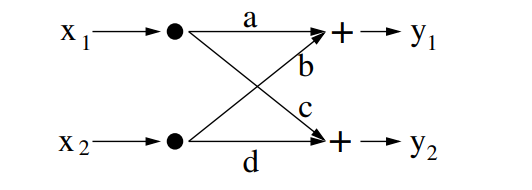
\includegraphics[width=0.6\textwidth]{graph/t1.png}
\end{figure}

Reversing all arrows and exchanging vertices $+$ and $\bullet$ yield the following graph:

\begin{figure}[h]
    \centering
    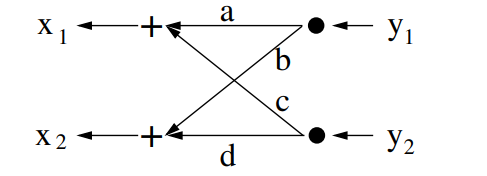
\includegraphics[width=0.6\textwidth]{graph/t2.png}
\end{figure}
Taking $y_1$, $y_2$ as input, it computes the transposed map $x_1 = ay_1 + cy_2, x_2 = by_1 + dy_2$.

In this section, we transpose the Brakedown linear code to get a reverse encoding algorithm. Figure \ref{fig:lc} is the construction of Brakedown linear code. And figure \ref{fig:lc-rev} is the reversed construction.


\begin{figure}[h]
\centering
\begin{tikzpicture}


\draw [-stealth](0,0) node[anchor=east] {input} -- (1,0) node[anchor=west]{\textbf{.}};
\draw [-stealth](1.4,0) -- (5.4,0);

\draw (5.6,1) rectangle node{x} (6.2,-1.0);
\draw (5.6,-1.0) rectangle node{z} (6.2,-3.0);
\draw (5.6,-3.0) rectangle node{v} (6.2,-5.0);

\draw [-stealth](1.2,-0.2) -- node[below left] {$A$} (2.2,-1.8) node[anchor=north west]{\textbf{.}};
\draw [-stealth](2.6,-2) -- node[above] {Enc} (3.8,-2) node[anchor=west]{\textbf{.}};
\draw [-stealth](4.2,-2) -- (5.4,-2);
\draw [-stealth](4.0,-2.2) -- node[below left] {$B$} (5.4,-4);
\draw [-stealth](6.4,-2) -- (7.4,-2) node[anchor=west]{output};

\end{tikzpicture}
\caption{Brakedown Linear Code}
\label{fig:lc}
\end{figure}



\begin{figure}[h]
\centering
\begin{tikzpicture}


\draw [stealth-](0,0) node[anchor=east] {output} -- (1,0) node[anchor=west]{\textbf{+}};
\draw [stealth-](1.45,0) -- (5.4,0);

\draw (5.6,1) rectangle node{x} (6.2,-1.0);
\draw (5.6,-1.0) rectangle node{z} (6.2,-3.0);
\draw (5.6,-3.0) rectangle node{v} (6.2,-5.0);

\draw [stealth-](1.2,-0.2) -- node[below left] {$A^T$} (2.2,-1.8);
\draw [stealth-](2.6,-2) node[anchor=east]{\textbf{+}} -- node[above] {Enc$^{-1}$} (3.8,-2) node[anchor=west]{\textbf{+}};
\draw [stealth-](4.25,-2) -- (5.4,-2);
\draw [stealth-](4.0,-2.2) -- node[below left] {$B^T$} (5.4,-4);
\draw [stealth-](6.4,-2) -- (7.4,-2) node[anchor=west]{input};

\end{tikzpicture}
\caption{Reversed Brakedown Linear Code}
\label{fig:lc-rev}
\end{figure}


\section{Construction}

This construction transforms an existing linear code into another linear code. The linear code constructed will have better relative distance and is equipped with the zero-knowledge property.

\subsection{Redistribution}

Given the normal encoding function \textbf{Enc()} and message $x$, we first compute the codeword $y = \textbf{Enc}(x) \in \mathbb{F}^n$. Then a random expander graph $G = (L, R, E)$ with degree $\Delta$ satisfying lemma \ref{lemma:randomgraph} will be generated. We will redistribute the symbols in $y$ according to $G$. More concretely, for every $i \in [n]$ and $j \in [\Delta]$, let $\gamma(i, j)$ be the index of the $j$-th vertex in $R$. The $(i - 1) \cdot \Delta + j$-th entry of $z$ is defined to be the $y_{\gamma(i, j)}$.

\subsection{Randomization}

Given $z \in \mathbb{F}^{n \cdot \Delta}$, we generate a random block diagonal matrix $H$ with $n$ blocks each of size $\Delta \cdot \Delta$. We compute $v = H \cdot z \in \mathbb{F}^{n \cdot \Delta}$.

\subsection{Reverse Encoding}

Given the reverse encoding function $\textbf{Enc}^{\top}$, the final output is $w = \textbf{Enc}^{\top}(v)$.

\section{Performance}

\begin{figure}[h]
    \centering
    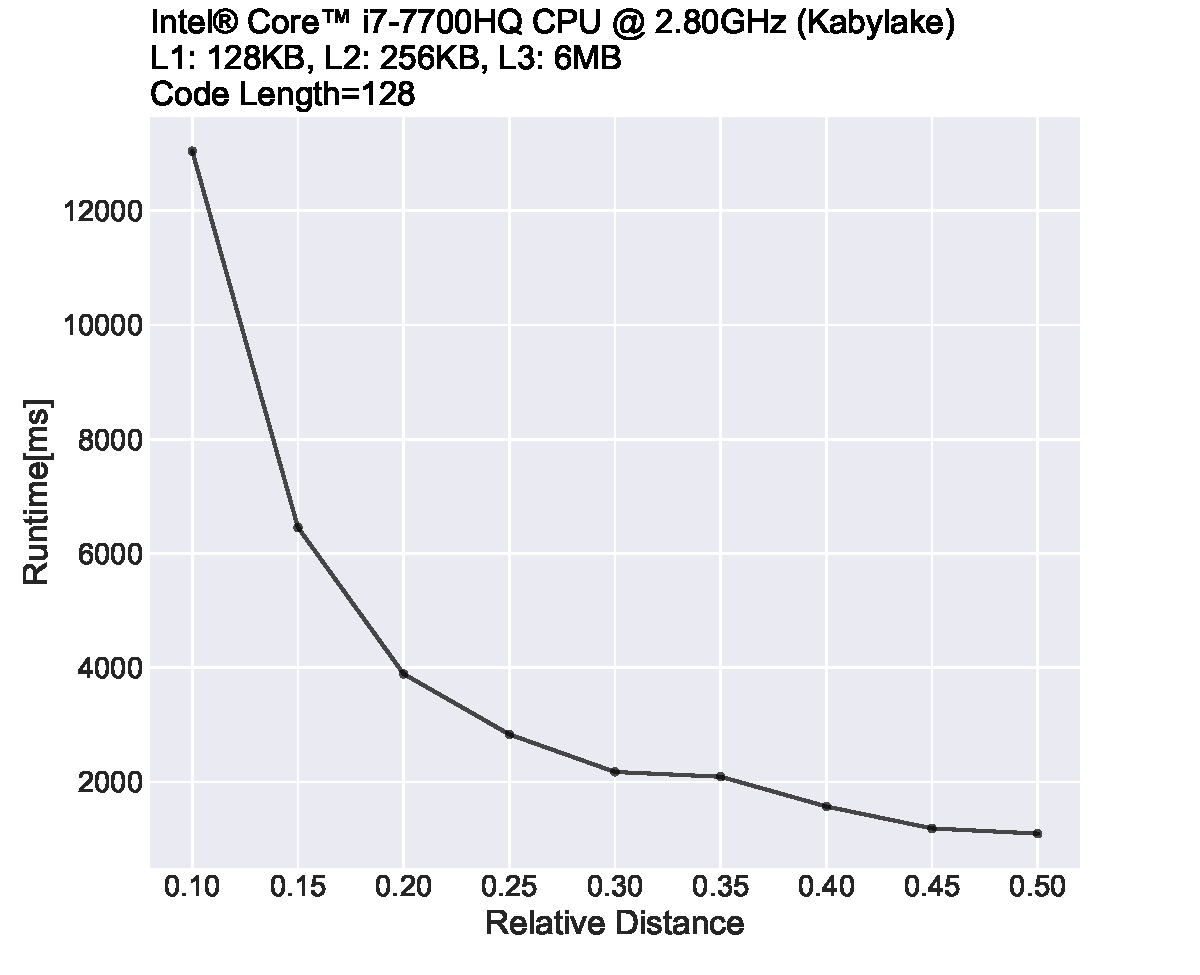
\includegraphics[width=1\textwidth]{graph/degree.pdf}
    \caption{Runtime of Redistribution and Randomization Step}
    \label{fig:degree}
\end{figure}


We have implemented the above construction. We measure the runtime required for the redistribution step and the randomization step, whose execution is irrelevant to the actual underlying linear code.


According to lemma \ref{lemma:randomgraph2}, the degree of the expander graph is very sensitive to the relative distance of underlying linear code. The larger the relative distance, the smaller the degree. And larger degree will cause the algorithm more time-consuming.

Figure \ref{fig:degree} presents the relation between relative distance and runtime. As the relative distance approaches 0.1, the runtime increases dramatically. And even for a larger relative distance, the construction is still significantly slower than the original linear code, making this construction unacceptable in practice.

\section{Improvement}

The performance of our zero-knowledge linear code construction suffers from the degree of underlying random expander graph. Recently, we notice an idea presented in \cite{orion} that might solve this problem. They propose a new algorithm to test whether a random bipartite graph is a lossless expander graph or not based on the densest subgraph algorithm, which helps to sample lossless expanders with an overwhelming probability.

We can prove a graph is not an expander graph by providing one counter-example. The densest-subgraph algorithm used by this detection algorithm can help us to find the counter-example efficiently.
Basically, if the graph is not a good expander graph, the detection algorithm in \cite{orion} can identify this situation with some probability $p$ using a random input $r$. And if the graph is a good expander graph, the detection algorithm will not falsely identify it (no false positive). Then we can run this detection algorithm $\lambda$ times with different random inputs and amplify the detection probability to $1 - (1 - p)^\lambda$. Additionally, if we find the graph is not a good expander graph, then we can simply discard it and generate a new random graph.


And if we have an efficient detection algorithm like this, we can randomly generate the expander graph with a much smaller degree $d$ and run the detection algorithm on it. Depending on the output of the detection algorithm, we can either be convinced that it is a good expander graph or we can re-run the generation algorithm one more time. The redistribution step in our construction will be much more efficient with such a small degree expander graph.


\begin{definition}
\label{definition:randomgraph2}

Let $\delta > 0$ and $0 < \epsilon < 1$ be a constant. Let $G=(L, R, E)$ be a $d$-regular bipartite graph with $|L| = n$. Graph $G$ is an expander graph if the following expansion property is satisfied:

    \begin{itemize}
        \item Expansion: For every set $X \subset L$ with $|X| \le \frac{\delta n}{d}$, if $Y$ is the set of neighbors of $X$ in $G$, then $|Y| \ge (1 - \epsilon) d |X|$.
    \end{itemize}

\end{definition}

However, due to the difference in expander graph definition, it is fundamentally not possible to reuse this densest-subgraph based detection algorithm in our project to improve efficiency. Definition \ref{definition:randomgraph2} is the expander graph used in \cite{orion} and lemma \ref{lemma:randomgraph} is the expander graph used in our project. The key difference is their expansion property. Informally speaking, definition \ref{definition:randomgraph2} needs the graph to have good expansion properties when we choose a small subset of vertices. And lemma \ref{lemma:randomgraph} needs the graph to have good expansion properties when we choose a large subset of vertices. The counter-example found by the densest-subgraph algorithm may have a small subset of vertices. And this is enough to be a good counter-example according to definition \ref{definition:randomgraph2}, but not enough according to lemma \ref{lemma:randomgraph}.

Therefore, it remains unclear how to improve the efficiency of this construction. And using a method similar to one-time-pad encryption, we can add zero-knowledge property into the polynomial commitment scheme. And it is practical and efficient compared with the alternative approach.